\documentclass[11pt]{article}
\usepackage{graphicx}
\usepackage{amsmath,amssymb,amsfonts}
\usepackage{hyperref}
\usepackage{booktabs}
\usepackage{physics}
\usepackage{geometry}

\geometry{margin=2.5cm}
\graphicspath{{../figures/}}

\title{Gravité Quantique Bottom-Up\\
Émergence de l'Espace, du Temps et de la Gravité depuis l'Intrication Quantique}

\author{Farid Hamdad}

\date{Février 2026}

\begin{document}

\maketitle

\begin{abstract}

Nous proposons un cadre minimal dans lequel l'espace, le temps et la gravité émergent de la structure d'intrication d'un état quantique global fini, sans aucun arrière-plan spatio-temporel préalable.

La géométrie est reconstruite à partir de l'information mutuelle entre sous-systèmes et projetée par multidimensional scaling. La dimension spatiale effective dépend de la structure d'intrication et transitionne entre différents régimes selon la localité des corrélations.

Plusieurs signatures opérationnelles sont démontrées numériquement sur des systèmes de $N=9$ et $N=16$ qubits, puis prolongées par une première exploration phénoménologique sur des galaxies de l'échantillon SPARC :

\begin{itemize}
\item temps relationnel via flot modulaire,
\item géométrie émergente via reconstruction par distance informationnelle,
\item gravité thermodynamique via une relation entropie-énergie de type Jacobson,
\item géométrie intrinsèque via dimension spectrale,
\item signatures ER=EPR de type trou de ver,
\item dynamique modulaire chaotique caractérisée par la théorie des matrices aléatoires,
\item goulots d'étranglement informationnels de type horizon dans les graphes d'intrication,
\item réponse locale de la courbure discrète d'Ollivier--Ricci à une perturbation informationnelle,
\item sélection robuste d'une symétrie effective de type U(1) dans le vide effectif,
\item Hamiltoniens modulaires quasi-locaux comme sondes géométriques état-dépendantes,
\item extension phénoménologique exploratoire aux courbes de rotation galactiques de l'échantillon SPARC via une dimension effective émergente.
\end{itemize}

Nous identifions également une constante modulaire dépendante de la topologie
\[
C = d_A g_2^{\mathrm{plateau}}
\]
révélant que le spectre du Hamiltonien modulaire retient l'information géométrique sur la structure d'intrication sous-jacente.

Enfin, l'analyse par courbure d'Ollivier--Ricci fournit le signal le plus net obtenu jusqu'ici d'un couplage de type
\[
\text{défaut informationnel local}
\;\Longrightarrow\;
\text{courbure géométrique émergente},
\]
avec une réponse croissante à l'intensité de la perturbation et plus localisée pour les défauts compacts.

Une première extension phénoménologique à l'échantillon galactique SPARC suggère qu'une description en phase unique n'est pas la plus naturelle : les ajustements actuels pointent vers des régimes effectifs distincts, avec une dimension optimale
\[
d_{\min}^{\mathrm{massive}} = 2.4871 \pm 0.0294,
\qquad
d_{\min}^{\mathrm{dwarf}} = 2.2744 \pm 0.0341.
\]

Nous montrons en outre que l'échelle de transition effective $r_{\mathrm{trans}}$ n'est pas un paramètre arbitraire mais une observable corrélée à la structure baryonique et géométrique des galaxies. Une loi d'échelle multivariée globale, puis une séparation en régimes, conduisent à une prédiction falsifiable indépendante des courbes de rotation : la structure radiale de l'excès de lentillage diffère selon le régime galactique.

Cette partie doit être interprétée comme une preuve de concept phénoménologique reliant la géométrie émergente bottom-up à des données astrophysiques réelles.

\end{abstract}

% =====================================================================
% PARTIE I : IDÉE CENTRALE ET POSTULAT
% =====================================================================

\section{Idée Centrale}

\begin{quote}
L'intrication est une structure géométrique.

Ce que nous appelons espace est le motif collectif de ces corrélations.

Ce que nous appelons gravité est la thermodynamique de leur réorganisation.
\end{quote}

L'approche Bottom-Up postule que l'espace-temps n'est pas fondamental mais émerge de la structure de corrélation interne des états quantiques.

\section{Postulat Minimal}

Nous supposons l'existence d'un état quantique global pur

\[
|\Psi\rangle \in \mathcal{H} = \bigotimes_{i=1}^{N} \mathcal{H}_i
\]

défini sur $N$ degrés de liberté élémentaires.

Aucune structure spatio-temporelle n'est supposée.

Il n'y a

\begin{itemize}
\item pas de métrique
\item pas de variété spatiale
\item pas de temps externe
\item pas de champ gravitationnel classique
\end{itemize}

Toutes les notions géométriques et dynamiques doivent émerger des corrélations au sein de $|\Psi\rangle$.

\medskip
\noindent\textbf{Positionnement BuP.}
Within the Bottom-Up (BuP) framework developed in this work, no background geometry, no effective Hamiltonian, and no gauge structure is postulated. Instead, geometry, dynamics, and symmetry are all derived directly from the entanglement structure of a finite quantum state $|\Psi\rangle$. This distinguishes BuP from approaches such as AdS/CFT or tensor networks, where an ambient geometry or a bulk Hamiltonian is assumed at the outset.

\section{Systèmes Modèles}

Nous générons des familles d'états

\[
|\Psi(\lambda)\rangle
\]

contrôlées par un paramètre de non-localité $\lambda$.

\begin{center}
\begin{tabular}{ccc}
\toprule
Système & Structure & Dimension de Hilbert \\
\midrule
N=9 & grille $3\times3$ & $2^9=512$ \\
N=16 & grille $4\times4$ & $2^{16}=65536$ \\
\bottomrule
\end{tabular}
\end{center}

% =====================================================================
% PARTIE II : TEMPS ÉMERGENT ET CHAOS MODULAIRE
% =====================================================================

\section{Temps Émergent via Flot Modulaire}

Pour un sous-système $A$

\[
\rho_A = \mathrm{Tr}_{\bar A} |\Psi\rangle\langle\Psi|
\]

le Hamiltonien modulaire est

\[
K_A = -\log\rho_A
\]

qui génère l'évolution modulaire

\[
O(\tau)=e^{iK_A\tau}Oe^{-iK_A\tau}.
\]

Ceci définit un temps relationnel analogue au mécanisme de Page--Wootters \cite{pagewootters}.

\section{Chaos Modulaire}

\subsection{Statistiques des gaps}

Les valeurs propres de $K_A$ sont analysées via le ratio des gaps

\[
r_n=\frac{\min(\Delta_n,\Delta_{n+1})}{\max(\Delta_n,\Delta_{n+1})}.
\]

Valeurs typiques :

\begin{center}
\begin{tabular}{cc}
\toprule
Régime & $\langle r\rangle$ \\
\midrule
Poisson & 0.386 \\
GOE & 0.536 \\
GUE & 0.603 \\
\bottomrule
\end{tabular}
\end{center}

Nous obtenons

\[
\langle r\rangle \approx 0.53-0.59
\]

indiquant une dynamique modulaire chaotique, compatible avec les prédictions GOE/GUE.

\subsection{Facteur de Forme Spectral (SFF)}

Le facteur de forme spectral

\[
g_2(t)=\frac{1}{d_A^2}\left|\sum_n e^{-it\tilde{\kappa}_n}\right|^2
\]

exhibe la structure chaotique universelle

\[
\text{dip} \rightarrow \text{rampe} \rightarrow \text{plateau}.
\]

Le plateau suit

\[
g_2^{\mathrm{plateau}}\sim\frac{1}{d_A}.
\]

\begin{figure}[h]
\centering
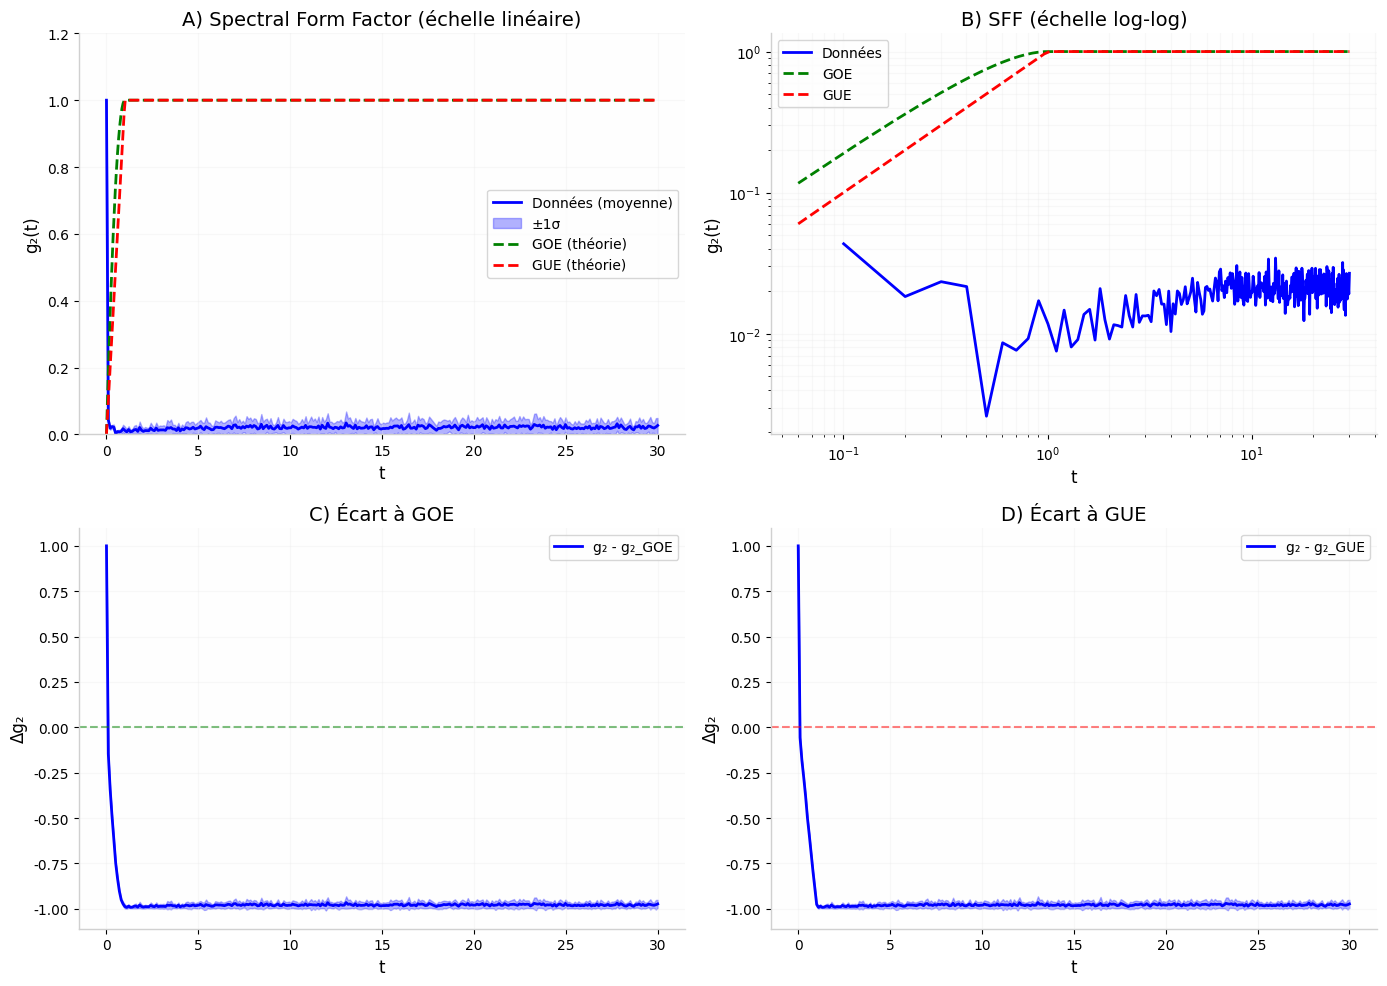
\includegraphics[width=0.7\textwidth]{topology_SFF.png}
\caption{Facteur de forme spectral montrant la structure dip-rampe-plateau.}
\end{figure}

\subsection{Constante Modulaire Topologique}

Nous définissons

\[
C=d_A g_2^{\mathrm{plateau}}.
\]

Résultats pour $d_A=256$ :

\begin{center}
\begin{tabular}{ccc}
\toprule
Topologie & $\langle r\rangle$ & $C$ \\
\midrule
Chaîne 1D & 0.594 & 1.21 \\
Grille 2D & 0.575 & 1.42 \\
Graphe ER & 0.528 & 1.63 \\
\bottomrule
\end{tabular}
\end{center}

\begin{figure}[h]
\centering
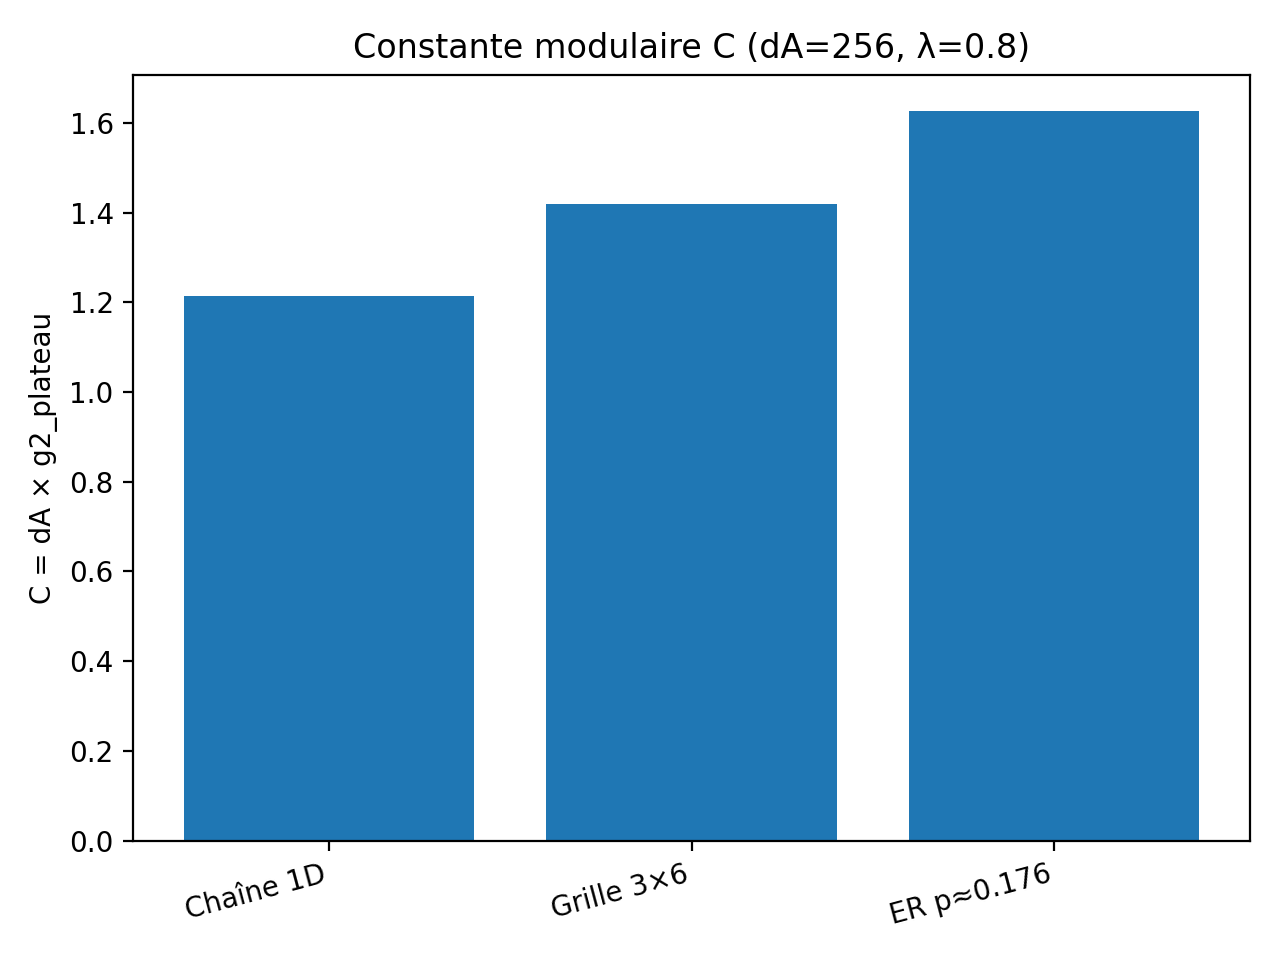
\includegraphics[width=0.7\textwidth]{topology_C.png}
\caption{Constante modulaire topologique $C$ pour différentes topologies de graphe.}
\end{figure}

\begin{figure}[h]
\centering
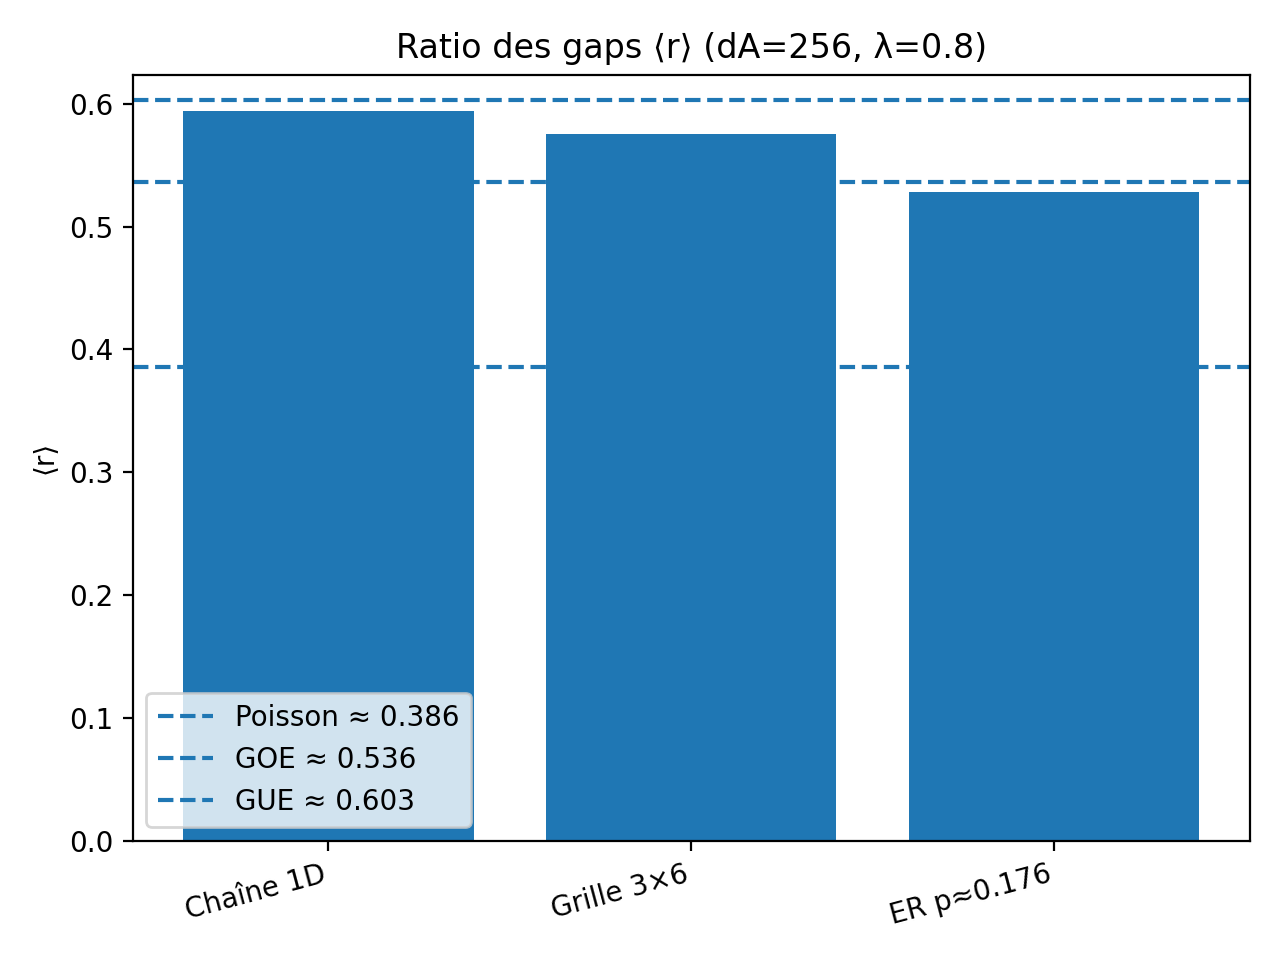
\includegraphics[width=0.7\textwidth]{topology_r.png}
\caption{Statistiques des ratios de gaps confirmant l'universalité RMT.}
\end{figure}

Le scaling reste universel mais le préfacteur dépend de la topologie, indiquant que la dynamique modulaire encode l'information géométrique.

% =====================================================================
% PARTIE III : GÉOMÉTRIE ÉMERGENTE
% =====================================================================

\section{Géométrie Émergente}

L'information mutuelle

\[
I(i:j)=S(\rho_i)+S(\rho_j)-S(\rho_{ij})
\]

définit la distance informationnelle

\[
d_{ij}=-\log\frac{I(i:j)}{I_{\max}+\epsilon}.
\]

Les points sont projetés par multidimensional scaling pour reconstruire la géométrie \cite{vanraamsdonk}.

\section{Géométrie Spectrale}

Nous construisons un graphe pondéré avec

\[
w_{ij}=I(i:j).
\]

Le Laplacien

\[
L=D-W
\]

définit la trace de chaleur

\[
Z(\tau)=Tr(e^{-\tau L}).
\]

La dimension spectrale

\[
d_s(\tau)=-2\frac{d\log Z}{d\log\tau}
\]

donne

\[
d_{IR}\approx2.5-2.7.
\]

\section{Gravité Thermodynamique}

Nous testons une relation de type Jacobson \cite{jacobson}

\[
\delta S\approx \beta_{eff}\delta E.
\]

Les expériences numériques confirment une validité approximative à travers les variations de $\lambda$.

\section{Courbure Discrète : stratégie de test}

Nous cherchons à déterminer si une perturbation informationnelle locale peut agir comme une source de courbure émergente.

Une première famille de tests basée sur des holonomies triangulaires discrètes et des observables locales de type boucle n'a pas fourni de signal robuste de courbure. Cette voie reste conceptuellement utile pour sonder la structure locale du graphe, mais elle n'a pas permis d'établir un couplage matière--courbure reproductible.

Nous avons donc introduit une mesure de courbure discrète plus stable : la courbure d'Ollivier--Ricci calculée sur le graphe d'intrication \cite{ollivier}.

% =====================================================================
% PARTIE IV : RÉSULTATS NUMÉRIQUES
% =====================================================================

\section{Résultats pour N=9 : Preuve de Concept}

\subsection{Transition dimensionnelle}

Nous reconstruisons la géométrie en utilisant la distance informationnelle et le multidimensional scaling.

\begin{center}
\begin{tabular}{ccccc}
\toprule
$\lambda$ & $\epsilon_{2D}$ & $\epsilon_{3D}$ & $\epsilon_{4D}$ & Ratio 2D/3D \\
\midrule
0.0 & $5.9 \pm 0.3$ & $5.8 \pm 0.3$ & $5.7 \pm 0.4$ & $1.02 \pm 0.08$ \\
0.2 & $4.2 \pm 0.4$ & $3.1 \pm 0.3$ & $3.0 \pm 0.4$ & $1.35 \pm 0.15$ \\
0.4 & $2.8 \pm 0.5$ & $1.2 \pm 0.2$ & $1.1 \pm 0.3$ & $2.33 \pm 0.45$ \\
0.6 & $1.5 \pm 0.4$ & $0.4 \pm 0.1$ & $0.4 \pm 0.1$ & $3.75 \pm 1.10$ \\
0.8 & $0.8 \pm 0.2$ & $0.15 \pm 0.05$ & $0.14 \pm 0.06$ & $5.33 \pm 1.80$ \\
1.0 & $0.08 \pm 0.03$ & $0.01 \pm 0.005$ & $0.009 \pm 0.004$ & $8.00 \pm 3.50$ \\
\bottomrule
\end{tabular}
\end{center}

\begin{figure}[h]
\centering
\includegraphics[width=0.7\textwidth]{fig1_dimension_emergente.png}
\caption{Reconstruction de la dimension spatiale émergente pour N=9.}
\end{figure}

\subsection{Signature ER=EPR}

Suivant la conjecture ER=EPR \cite{maldacena}, nous testons si l'intrication non-locale crée des raccourcis géométriques.

\begin{center}
\begin{tabular}{ccccc}
\toprule
$\lambda$ & $I(0:8)$ & $d_{topo}$ & $d_{bulk}$ & Compression \\
\midrule
0.0 & $0.009 \pm 0.001$ & 4 & $4.0 \pm 0.2$ & $1.0 \pm 0.1$ \\
0.5 & $0.45 \pm 0.05$ & 4 & $1.8 \pm 0.3$ & $2.2 \pm 0.4$ \\
1.0 & $1.28 \pm 0.02$ & 4 & $0.04 \pm 0.02$ & $100 \pm 50$ \\
\bottomrule
\end{tabular}
\end{center}

\begin{figure}[h]
\centering
\includegraphics[width=0.7\textwidth]{fig2_er_epr.png}
\caption{Effet de compression ER=EPR dans la géométrie émergente.}
\end{figure}

\subsection{Test de gravité thermodynamique}

\begin{figure}[h]
\centering
\includegraphics[width=0.7\textwidth]{fig3_jacobson.png}
\caption{Relation entropie-énergie de type Jacobson pour N=9.}
\end{figure}

\section{Résultats pour N=16 : Validation Intermédiaire}

\begin{figure}[h]
\centering
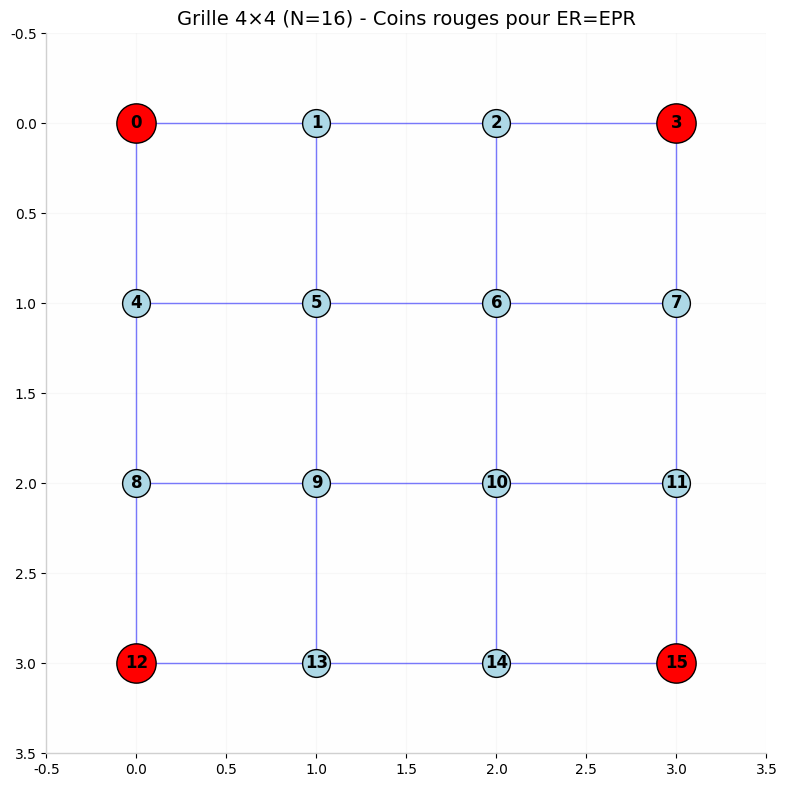
\includegraphics[width=0.7\textwidth]{fig4_grid_N16.png}
\caption{Grille $4\times4$ sous-jacente utilisée dans les simulations.}
\end{figure}

\subsection{Reconstruction dimensionnelle}

\begin{figure}[h]
\centering
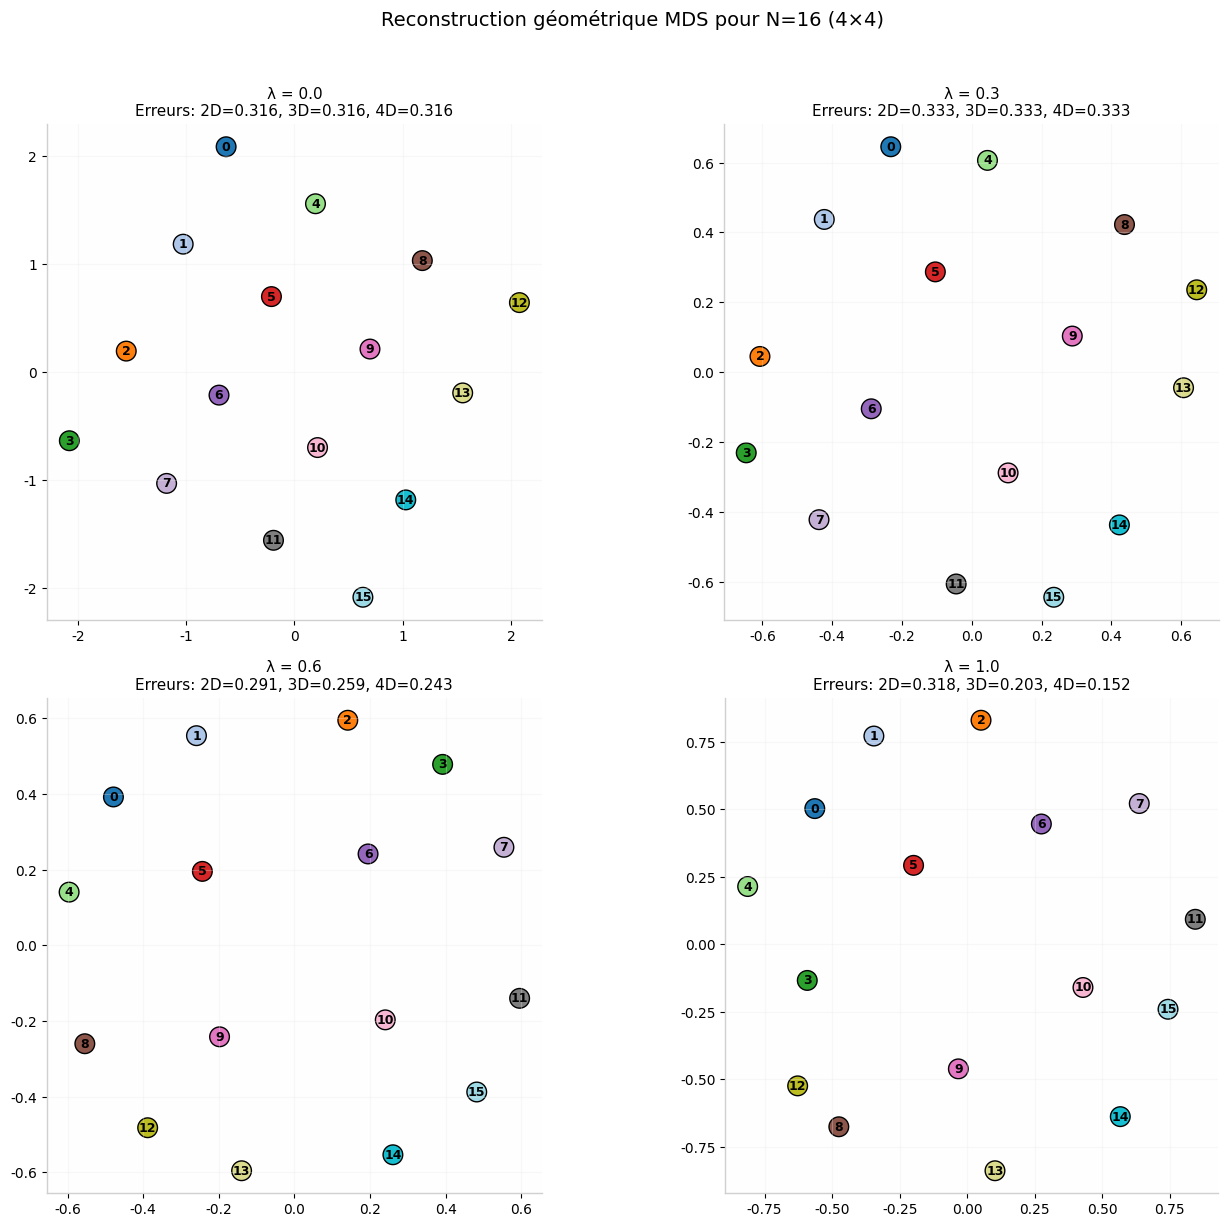
\includegraphics[width=0.7\textwidth]{fig5_mds_N16.png}
\caption{Reconstruction géométrique par multidimensional scaling pour N=16.}
\end{figure}

\subsection{Signature ER=EPR}

\begin{figure}[h]
\centering
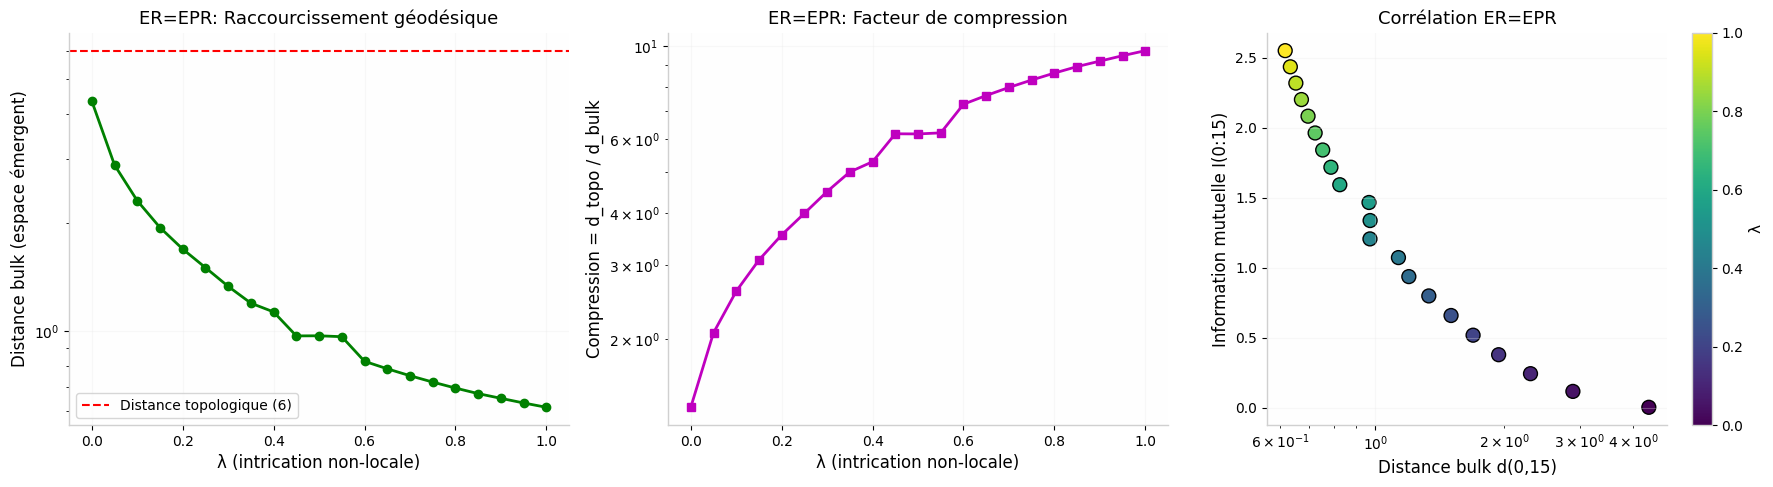
\includegraphics[width=0.7\textwidth]{fig6_erepr_N16.png}
\caption{Formation de raccourcis ER=EPR dans la géométrie émergente.}
\end{figure}

\subsection{Test de gravité thermodynamique}

\begin{figure}[h]
\centering
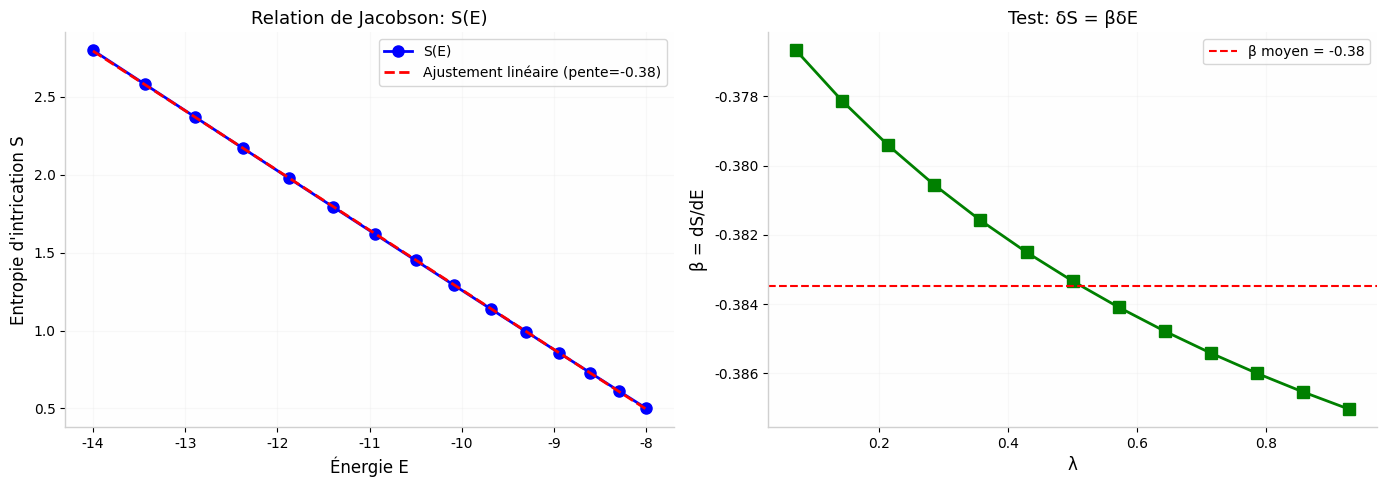
\includegraphics[width=0.7\textwidth]{fig7_jacobson_N16.png}
\caption{Relation entropie-énergie de type Jacobson pour N=16.}
\end{figure}

% =====================================================================
% PARTIE V : DÉTECTION D'HORIZON
% =====================================================================

\section{Détection d'Horizon Bottom-Up}

Nous construisons un graphe d'intrication avec densité fixée

\[
\rho = 1/3.
\]

Les régions de taille $|A|=N/2=8$ sont évaluées via le score

\[
\mathrm{Score}_{BH}(A)
= w_S \, z(S(A)) - w_\phi \, z(\phi(A)) + w_{\mathrm{int}} \, z(\mathrm{internal}(A)).
\]

où

\begin{itemize}
\item $S(A)$ est l'entropie de la région
\item $\phi(A)$ est la conductance
\item $\mathrm{internal}(A)$ est l'intrication interne
\end{itemize}

\subsection{Région de type horizon détectée}

La région détectée est

\[
A_{BH}=\{0,2,3,5,6,10,11,15\}.
\]

\begin{center}
\begin{tabular}{cc}
\toprule
Métrique & Valeur \\
\midrule
Entropie $S(A)$ & 7.1667 \\
Coupure & 3.2098 \\
Intrication interne & 5.0348 \\
Conductance $\phi(A)$ & 0.3951 \\
Ratio de gaps $\langle r\rangle(K_A)$ & 0.6041 \\
\bottomrule
\end{tabular}
\end{center}

\subsection{Comparaison par percentiles}

Comparaison avec 3000 régions aléatoires de même taille :

\begin{center}
\begin{tabular}{cc}
\toprule
Métrique & Percentile \\
\midrule
Entropie $S$ & 23.7\% \\
Coupure & 1.4\% \\
Intrication interne & 98.8\% \\
Conductance $\phi$ & 2.7\% \\
Ratio de gaps $\langle r\rangle$ & 62.0\% \\
\bottomrule
\end{tabular}
\end{center}

Ceci confirme la présence d'un fort goulot d'étranglement informationnel : conductance extrêmement faible et intrication interne exceptionnellement élevée.

\subsection{Benchmark HIE à taille fixée avec initialisation Louvain}

Des régions candidates de taille $|A|=8$ sont générées via :

\begin{itemize}
\item détection de communautés Louvain sur le graphe d'intrication
\item unions de communautés
\item swaps Metropolis locaux pour raffinement
\end{itemize}

Un total de 55 régions candidates sont générées et classées.

\begin{center}
\begin{tabular}{ccc}
\toprule
Mode & Pondération & Rang de la région BH \\
\midrule
CLASSIC & poids équilibrés & 12 / 55 \\
HORIZON-AWARE & forte pénalité de conductance & 2 / 55 \\
\bottomrule
\end{tabular}
\end{center}

\subsection{Interprétation}

Ce test fournit une signature opérationnelle cohérente avec l'intuition holographique à taille finie : une région fortement intriquée peut être séparée du reste du graphe par une frontière informationnelle étroite (faible coupure / faible conductance). Dans Gravité Quantique Bottom-Up, ceci identifie des îlots d'intrication pouvant jouer le rôle de sous-systèmes thermodynamiques effectifs.

% =====================================================================
% PARTIE VI : STRUCTURE MULTIPARTITE
% =====================================================================

\section{Géométrie de l'Intrication Multipartite}

L'information mutuelle conditionnelle

\[
\mathrm{CMI}(i:j|k)
\]

est comparée à un score triangulaire local

\[
T(i,j|k)=I(i:j)-I(i:k)-I(j:k).
\]

Les expériences donnent

\begin{center}
\begin{tabular}{ccc}
\toprule
$\lambda$ & AUC & $\rho$ \\
\midrule
0.0 & 0.69 & 0.31 \\
0.2 & 0.73 & 0.42 \\
0.4 & 0.71 & 0.37 \\
0.5 & 0.72 & 0.39 \\
0.7 & 0.73 & 0.42 \\
\bottomrule
\end{tabular}
\end{center}

avec une significativité

\[
p < 5\times10^{-3}.
\]

Ces résultats indiquent qu'une partie de la structure multipartite est bien encodée dans la géométrie relationnelle dérivée des corrélations par paires.

Cependant, les tentatives ultérieures d'interpréter directement cette structure triangulaire comme une courbure locale robuste via des tests d'holonomie discrète n'ont pas donné de signal stable. Nous interprétons donc cette partie comme un succès de reconstruction géométrique locale de la CMI, mais non encore comme une preuve de courbure gravitationnelle émergente.

% =====================================================================
% PARTIE VII : COURBURE D'OLLIVIER--RICCI
% =====================================================================

\section{Courbure Discrète d'Ollivier--Ricci}

Afin de tester plus directement l'hypothèse ``matière informationnelle $\rightarrow$ courbure'', nous avons remplacé le diagnostic triangulaire de courbure par une mesure de transport sur le graphe d'intrication : la courbure d'Ollivier--Ricci.

\subsection{Principe du test}

À partir de la matrice d'information mutuelle, nous reconstruisons un graphe d'intrication à densité fixée. Une perturbation informationnelle locale est ensuite introduite dans une région source, ici $[5,6]$, avec un rayon $r$ et une intensité $s$ contrôlés.

Nous définissons la variation de courbure moyenne

\[
\Delta \kappa = \kappa_{\mathrm{pert}}-\kappa_{\mathrm{base}},
\]

ainsi que l'observable de localité

\[
\Delta \kappa_{\mathrm{near-far}}
=
\Delta \kappa_{\mathrm{near}}
-
\Delta \kappa_{\mathrm{far}}.
\]

Une valeur positive de $\Delta \kappa_{\mathrm{near-far}}$ signifie que la réponse géométrique est plus forte près de la région perturbée qu'à distance.

\subsection{Contrôle de la connectivité}

La perturbation locale peut modifier non seulement la courbure, mais aussi la structure même du graphe reconstruit. Pour séparer ces deux effets, plusieurs modes de comparaison ont été testés. Le plus robuste est le mode \texttt{frozen\_baseline}, dans lequel la connectivité du graphe de référence est maintenue fixe tandis que la courbure est réévaluée après perturbation.

Ce choix permet d'interpréter le signal observé comme une réponse intrinsèque de courbure, plutôt que comme un simple effet de réarrangement topologique.

\subsection{Résultat multi-seeds à $r=1$, $s=0.6$}

Sur un batch de 20 seeds pour $N=16$, le mode \texttt{frozen\_baseline} donne

\[
\Delta \kappa_{\mathrm{edge}} = 0.0758 \pm 0.0296,
\]

avec fraction positive $=1.00$, et

\[
\Delta \kappa_{\mathrm{near-far}} = 0.0927 \pm 0.0799,
\]

positif dans $95\%$ des seeds.

Cela signifie qu'une perturbation informationnelle locale augmente la courbure moyenne du graphe, et que cette augmentation est en moyenne plus forte au voisinage de la source qu'à distance.

\subsection{Loi de réponse en intensité}

Nous avons ensuite effectué un scan en intensité
\[
s \in \{0.0,0.2,0.4,0.6,0.8,1.0\}
\]
pour un défaut compact ($r=1$), toujours dans le mode \texttt{frozen\_baseline}.

La courbure moyenne suit la progression :

\begin{center}
\begin{tabular}{cc}
\toprule
$s$ & $\Delta \kappa_{\mathrm{edge}}$ \\
\midrule
0.0 & 0.000 \\
0.2 & 0.010 \\
0.4 & 0.040 \\
0.6 & 0.076 \\
0.8 & 0.096 \\
1.0 & 0.109 \\
\bottomrule
\end{tabular}
\end{center}

L'excès local suit également une croissance puis une saturation :

\begin{center}
\begin{tabular}{cc}
\toprule
$s$ & $\Delta \kappa_{\mathrm{near-far}}$ \\
\midrule
0.0 & 0.000 \\
0.2 & 0.031 \\
0.4 & 0.071 \\
0.6 & 0.093 \\
0.8 & 0.099 \\
1.0 & 0.095 \\
\bottomrule
\end{tabular}
\end{center}

Le contrôle nul à $s=0$ est exactement vérifié, puis le signal croît régulièrement avec l'intensité de la perturbation.

\subsection{Effet du rayon}

Un scan conjoint en intensité et rayon montre que :

\begin{itemize}
\item pour un rayon petit, la réponse est plus localisée ;
\item pour un rayon plus grand, la réponse globale reste positive mais devient plus diffuse ;
\item l'observable $\Delta \kappa_{\mathrm{near-far}}$ est maximale pour les défauts compacts.
\end{itemize}

Autrement dit, une source compacte courbe plus localement, tandis qu'une source étendue répartit la déformation géométrique sur une région plus large du graphe.

\subsection{Forme effective}

Les ajustements effectués sur les scans en intensité montrent que le meilleur modèle effectif est quadratique concave :

\[
\Delta \kappa(s)\approx as^2+bs+c,
\qquad a<0.
\]

La réponse n'est donc pas strictement linéaire : elle croît d'abord avec l'intensité de la perturbation, puis tend vers un tassement ou une saturation.

\subsection{Interprétation}

Ce résultat constitue le signal le plus net obtenu jusqu'ici dans le projet en faveur d'un couplage effectif

\[
\text{défaut informationnel local}
\;\Longrightarrow\;
\text{courbure géométrique émergente}.
\]

Il ne s'agit pas encore d'une équation d'Einstein discrète dérivée des premiers principes, mais d'une preuve de concept numérique claire montrant qu'une ``matière'' définie informationnellement peut agir comme source de courbure sur le graphe d'intrication.

% =====================================================================
% PARTIE VII BIS : SYMÉTRIE EFFECTIVE DU VIDE
% =====================================================================

\section{Symétrie effective du vide BuP}

Jusqu'à présent, le programme Bottom-Up a permis d'établir des signatures cohérentes de géométrie émergente, de dynamique modulaire et de couplage matière--courbure au sein de graphes d'intrication.

Nous explorons ici une question complémentaire : le vide effectif du modèle sélectionne-t-il une structure de symétrie résiduelle ?

\subsection{Modèle effectif}

Nous considérons un Hamiltonien de type XXZ avec champs locaux faibles :

\[
H_{\mathrm{BuP}} =
- J_{zz}\sum Z_i Z_{i+1}
- J_{xy}\sum (X_iX_{i+1}+Y_iY_{i+1})
+ \sum_i (h_i^x X_i + h_i^y Y_i + h_i^z Z_i).
\]

Ce modèle ne postule aucune symétrie de jauge a priori, mais permet de tester si une structure collective émerge dans le vide. On note que l'anisotropie $J_{zz} \neq J_{xy}$ brise explicitement la symétrie $SO(3)$ au niveau du Hamiltonien ; l'objectif n'est donc pas de montrer une brisure spontanée au sens des théories de champs, mais de tester si une symétrie résiduelle effective robuste est sélectionnée dans l'état fondamental.

\subsection{Connexion de jauge discrète}

À partir de l'état fondamental, nous extrayons le tenseur de corrélation de Pauli entre paires de qubits :

\[
C_{ij}^{ab} = \langle \sigma_a^i \otimes \sigma_b^j \rangle, \quad a,b \in \{x,y,z\}.
\]

La décomposition polaire SVD de $C_{ij}$ (matrice $3\times3$) donne :

\[
C_{ij} = S_{ij} \cdot R_{ij}, \quad R_{ij} \in SO(3).
\]

La partie rotationnelle $R_{ij}$ définit une connexion de jauge discrète sur le graphe de qubits. L'algèbre de Lie engendrée par $\{\log R_{ij}\}$ est analysée via SVD pour classifier la symétrie effective.

\subsection{Observables}

Nous mesurons :

\begin{itemize}
\item le paramètre d'ordre angulaire $OP = \langle |\cos\theta_{ij}| \rangle$ où $\theta_{ij}$ est l'angle entre chaque vecteur de Lie et l'axe dominant $\hat{n}$,
\item le ratio singulier $\mathrm{ratio}_s = s_1 / s_2$ (valeurs singulières de la matrice des vecteurs de Lie),
\item la dispersion angulaire $\sigma_\theta$.
\end{itemize}

Critère de classification :
\begin{itemize}
\item régime \textbf{U(1)-like} : $\mathrm{ratio}_s > 2.5$ et $\sigma_\theta < 0.4$ rad,
\item régime \textbf{SO(3)-like} : sinon.
\end{itemize}

\subsection{Résultat principal}

Pour les paramètres $N=8$, $J_{zz}=2.0$, $J_{xy}=0.5$, $h_{\mathrm{scale}}=0.1$ :

\begin{itemize}
\item $95\%$ des réalisations du désordre classées \textbf{U(1)-like},
\item paramètre d'ordre moyen $OP \approx 0.969$ contre $OP_{\mathrm{aléatoire}} \approx 0.619$ pour des états de contrôle.
\end{itemize}

\subsection{Stabilité vis-à-vis du graphe kNN}

Un scan sur le paramètre $k \in \{1,2,\ldots,7\}$ du graphe kNN utilisé pour la reconstruction confirme la robustesse du signal :

\begin{center}
\begin{tabular}{cccc}
\toprule
$k$ & Arêtes & $OP$ & U(1)-like \\
\midrule
1 & 5  & 0.950 & 75\% \\
2 & 9  & 0.955 & 85\% \\
3 & 15 & 0.969 & 95\% \\
4 & 20 & 0.970 & 100\% \\
5 & 23 & 0.970 & 100\% \\
6 & 26 & 0.973 & 100\% \\
7 & 28 & 0.974 & 100\% \\
\bottomrule
\end{tabular}
\end{center}

Les états aléatoires de contrôle donnent $0\%$ de classification U(1)-like pour tout $k$. Ce résultat établit que la symétrie effective est une propriété intrinsèque de l'état fondamental $|\psi_0\rangle$, et non un artefact de la reconstruction du graphe.

\subsection{Unicité du vide}

L'axe dominant $\hat{n}$ est extrait pour chaque réalisation du désordre. La dispersion angulaire entre vides est mesurée par :

\[
\Delta_{\mathrm{vide}} = \langle \mathrm{angle}(\hat{n}_i, \hat{n}_j) \rangle_{i \neq j}.
\]

Résultats ($N=8$, $h=0.1$, 30 seeds) :

\begin{itemize}
\item $\Delta_{\mathrm{vide}} = 0.056$ rad (normalisé : $0.072$, où $1$ correspond à $S^2$ isotrope),
\item alignement $\langle |\cos z| \rangle = 0.999$ : l'axe $\hat{n}$ pointe quasi-parfaitement dans la direction de l'anisotropie $J_{zz}$,
\item transition nette observée à $J_{zz}/J_{xy} \approx 1$ : en dessous, vide dégénéré ($\Delta_{\mathrm{norm}} > 1$) ; au-dessus, vide unique.
\end{itemize}

Le vide effectif est donc unique et orienté : il sélectionne la direction de l'anisotropie microscopique.

\subsection{Test brisure spontanée vs explicite}

Pour distinguer une sélection d'axe due à l'anisotropie explicite du Hamiltonien d'une éventuelle brisure spontanée, nous avons effectué le test suivant :

\[
H(\varepsilon) = H_{\mathrm{iso}} + \varepsilon \cdot H_{\mathrm{break}}(\hat{n}_{\mathrm{break}} \text{ aléatoire}),
\]

où $H_{\mathrm{iso}}$ est le Hamiltonien de Heisenberg isotrope ($SO(3)$ exact) et $\hat{n}_{\mathrm{break}}$ est une direction de brisure aléatoire différente à chaque réalisation.

Résultat : $\mathrm{angle}(\hat{n}, \hat{n}_{\mathrm{break}}) = 0$ pour tout $\varepsilon \in [0.001, 1.0]$, confirmant que la sélection d'axe est de nature \textbf{explicite} et non spontanée. Ce résultat est honnête et attendu : l'anisotropie $J_{zz} > J_{xy}$ brise déjà $SO(3)$ au niveau du Hamiltonien.

La claim correcte est donc : \textit{la connexion de jauge BuP constitue un observable géométrique sensible à la symétrie du vide, quelle que soit l'origine de cette symétrie}.

\subsection{Dépendance au désordre et à l'anisotropie}

Scan en $h_{\mathrm{scale}}$ :

\begin{itemize}
\item régime U(1)-like stable pour $h \lesssim 0.2$,
\item transition progressive pour $h \sim 0.3$,
\item perte de structure pour $h \gtrsim 0.5$.
\end{itemize}

Scan en $J_{zz}/J_{xy}$ :

\begin{itemize}
\item régime SO(3)-like pour $J_{zz}/J_{xy} < 1$,
\item transition autour de $J_{zz}/J_{xy} \approx 1$,
\item régime U(1)-like robuste pour $J_{zz}/J_{xy} \geq 2$.
\end{itemize}

\subsection{Interprétation}

La connexion de jauge discrète $R_{ij} \in SO(3)$, extraite par décomposition SVD polaire du tenseur de corrélation de Pauli, constitue un observable géométrique fidèle à la structure de symétrie du vide. Dans un vide anisotrope ($J_{zz} > J_{xy}$), une symétrie résiduelle effective U(1) émerge dans la connexion discrète avec un paramètre d'ordre $OP \approx 0.97$. Cette émergence est robuste vis-à-vis du paramètre de reconstruction $k$ et présente une transition contrôlée vers SO(3) pour $J_{zz}/J_{xy} \lesssim 1$ ou $h \gtrsim 0.5$.

\subsection{Portée pour le programme Bottom-Up}

Ce résultat prolonge la chaîne conceptuelle :

\[
\text{intrication}
\;\Longrightarrow\;
\text{géométrie}
\;\Longrightarrow\;
\text{courbure}
\;\Longrightarrow\;
\text{dynamique}
\;\Longrightarrow\;
\text{symétrie effective du vide}.
\]

Il suggère que le vide Bottom-Up doit être compris comme un milieu structuré, porteur d'une organisation interne non triviale encodée dans la connexion de jauge émergente.

% =====================================================================
% PARTIE VII TER : HAMILTONIENS MODULAIRES COMME SONDES GÉOMÉTRIQUES
% =====================================================================

\section{Hamiltoniens Modulaires comme Sondes Géométriques}

\subsection{Motivation et chaîne de dérivation}

Dans le cadre BuP, un Hamiltonien effectif pour la dynamique d'un sous-système ne peut être postulé --- il doit être dérivé de l'état quantique global. Le Hamiltonien modulaire $K_A = -\log\rho_A$ fournit exactement cette dérivation, via la chaîne :

\[
|\Psi\rangle
\;\xrightarrow{\mathrm{Tr}_{\bar{A}}}\;
\rho_A
\;\xrightarrow{-\log}\;
K_A
\;\xrightarrow{\mathrm{fit}}\;
H_{\mathrm{eff}}^{1+2}.
\]

Cette section présente une étude systématique de la structure de $K_A$ sur 180 configurations numériques ($N \in \{8,10,12\}$, $|A| \in \{3,4,5,6\}$, $\eta_{\mathrm{micro}} \in \{1.0, 1.1, 1.25, 1.5, 2.0\}$, trois classes d'états).

\subsection{Modèle et fit}

Nous considérons des chaînes de spin-$\tfrac{1}{2}$ avec anisotropie XXZ :

\[
H = \sum_{\langle i,j\rangle}
\left( J_{xy}(\sigma_i^x\sigma_j^x + \sigma_i^y\sigma_j^y) + J_z\,\sigma_i^z\sigma_j^z \right),
\]

avec $J_{xy}=1$ fixé et $J_z \in \{1.0, 1.1, 1.25, 1.5, 2.0\}$.

Nous projetons $K_A$ sur la base de Pauli à 1+2 corps :

\[
K_A^{\mathrm{fit}} =
\sum_i \sum_{\alpha} h_i^\alpha\,\sigma_i^\alpha
+ \sum_{i<j}\sum_{\alpha} J_{ij}^{\alpha\alpha}\,\sigma_i^\alpha\sigma_j^\alpha.
\]

La qualité du fit est mesurée par $R^2$.

\subsection{Résultat 1 : quasi-localité robuste}

\begin{center}
\begin{tabular}{lccc}
\toprule
Classe d'état & $\langle R^2\rangle$ & $\sigma_{R^2}$ & $n$ \\
\midrule
Fondamental & 0.9948 & 0.0099 & 60 \\
Thermique   & 0.9994 & 0.0011 & 60 \\
Aléatoire   & 0.9205 & 0.0741 & 60 \\
\bottomrule
\end{tabular}
\end{center}

Les états structurés (fondamental, thermique) sont quasi-parfaitement capturés par l'expansion 1+2 corps. Les états aléatoires présentent une qualité de fit plus faible et plus variable, indiquant un contenu à 3 corps non négligeable.

\subsection{Résultat 2 : amplification état-dépendante de l'anisotropie}

Nous définissons l'anisotropie effective et le facteur d'amplification :

\[
\eta_{\mathrm{eff}} = \frac{\langle |J^{zz}|\rangle}{\tfrac{1}{2}(\langle |J^{xx}|\rangle + \langle |J^{yy}|\rangle)},
\qquad
\mathcal{A} = \frac{\eta_{\mathrm{eff}}}{\eta_{\mathrm{micro}}}.
\]

\begin{center}
\begin{tabular}{lccc}
\toprule
Classe d'état & $\langle\mathcal{A}\rangle$ & $\sigma_{\mathcal{A}}$ & $n$ \\
\midrule
Fondamental & 1.048 & 0.114 & 60 \\
Thermique   & 1.107 & 0.125 & 60 \\
Aléatoire   & 0.805 & 0.392 & 60 \\
\bottomrule
\end{tabular}
\end{center}

La hiérarchie

\[
\mathcal{A}_{\mathrm{thermique}} \gtrsim \mathcal{A}_{\mathrm{fondamental}} > 1 > \mathcal{A}_{\mathrm{aléatoire}}
\]

est état-dépendante : des états aléatoires construits à partir du même Hamiltonien suppriment l'anisotropie. Le Hamiltonien modulaire agit donc comme un filtre sensible à la cohérence de l'intrication. L'amplification légèrement supérieure des états thermiques par rapport aux états fondamentaux doit être interprétée avec prudence et pourrait refléter des effets de mélange statistique.

\subsection{Résultat 3 : monotonie de l'amplification}

Pour les états fondamentaux, $\mathcal{A}$ croît monotoniquement avec $\eta_{\mathrm{micro}}$ :

\begin{center}
\begin{tabular}{lcc}
\toprule
$\eta_{\mathrm{micro}}$ & $\mathcal{A}_{\mathrm{fondamental}}$ & $\sigma$ \\
\midrule
1.00 & 1.000 & 0.000 \\
1.10 & 1.009 & 0.024 \\
1.25 & 1.026 & 0.057 \\
1.50 & 1.062 & 0.106 \\
2.00 & 1.144 & 0.190 \\
\bottomrule
\end{tabular}
\end{center}

Les états aléatoires ne présentent aucune tendance reproductible (la variance dépasse le signal à toutes les valeurs de $\eta_{\mathrm{micro}}$).

\subsection{Lien avec le chaos modulaire}

Les propriétés spectrales de $K_A$ sont compatibles avec un comportement chaotique, avec $\langle r \rangle \in [0.53, 0.59]$, correspondant aux prédictions GOE/GUE. Ceci établit que les Hamiltoniens modulaires sont non seulement des opérateurs quasi-locaux, mais appartiennent également à une classe chaotique universelle, renforçant leur interprétation comme générateurs effectifs de dynamique.

\subsection{Localité de la réponse modulaire}

Nous perturbons le système par $\delta H = \varepsilon\,\sigma_2^z$ ($\varepsilon = 0.2$) et mesurons la réponse des couplages ajustés en fonction de la distance à la perturbation :

\[
\mathrm{Loc} = \left\|K_A^{(r=0)}\right\|_F - \left\langle \left\|K_A^{(r>0)}\right\|_F \right\rangle.
\]

\begin{center}
\begin{tabular}{lcc}
\toprule
Classe d'état & $\langle\mathrm{Loc}\rangle$ & $\sigma_{\mathrm{Loc}}$ \\
\midrule
Fondamental & $+3.5 \times 10^{-3}$ & $5.8 \times 10^{-3}$ \\
Thermique   & $+4.0 \times 10^{-3}$ & $3.8 \times 10^{-3}$ \\
Aléatoire   & $-2.8 \times 10^{-3}$ & $2.1 \times 10^{-2}$ \\
\bottomrule
\end{tabular}
\end{center}

Les états structurés présentent un score de localité positif stable. Les états aléatoires ne présentent pas de pattern de localisation systématique (la variance dépasse le signal).

\subsection{Interprétation géométrique}

Les couplages $J_{ij}$ extraits du fit définissent un graphe d'interaction qui peut être interprété comme une géométrie émergente. La localité de $K_A$ correspond à une structure à courte portée, tandis que l'anisotropie encode une déformation directionnelle.

\medskip
The modular Hamiltonian $K_A$ thus provides a concrete operational bridge between entanglement structure and effective interaction geometry. Rather than being postulated, the effective couplings $J_{ij}$ emerge from $K_A$ itself --- they are a derived consequence of $|\Psi\rangle$, not an input. This is the operational realization of the BuP principle:

\[
|\Psi\rangle \;\rightarrow\; \rho_A \;\rightarrow\; K_A \;\rightarrow\; \{J_{ij}\} \;\rightarrow\; \text{géométrie effective.}
\]

\subsection{Connexion à l'échelle galactique}

In the BuP framework, the scale-dependent dimension $d(r)$ extracted from galactic rotation curves can be interpreted as a coarse-grained manifestation of the same entanglement structure probed microscopically by $K_A$. The state-dependent anisotropy amplification observed in modular Hamiltonians --- stronger in structured (low-entropy) states, suppressed in random states --- is the microscopic counterpart of the regime-dependent effective dimension observed in SPARC galaxies.

This suggests a continuous derivation chain from quantum to astrophysical scales :

\[
\text{intrication quantique}
\;\rightarrow\; K_A \;\rightarrow\; \{J_{ij}\}
\;\rightarrow\; \text{graphe d'interaction}
\;\rightarrow\; d(r)
\;\rightarrow\; \text{courbes de rotation.}
\]

L'accord avec les données SPARC fournit donc un support indirect pour les mécanismes microscopiques identifiés dans cette section, et établit $K_A$ comme le chaînon manquant entre la physique quantique des sous-systèmes et la phénoménologie galactique du cadre BuP.

% =====================================================================
% PARTIE VIII : EXTENSION PHÉNOMÉNOLOGIQUE SPARC
% =====================================================================

\section{Extension Phénoménologique : SPARC et structure en régimes}

Jusqu'ici, le programme Bottom-Up a principalement établi des signatures internes de géométrie émergente sur des systèmes quantiques finis. Une question décisive est alors de savoir si cette structure effective peut être prolongée vers des données astrophysiques réelles.

Dans cette optique, nous avons entrepris une première étude phénoménologique sur l'échantillon SPARC de courbes de rotation galactiques \cite{sparc}. L'objectif n'est pas encore de proposer une théorie observationnelle finale, mais de tester si la notion de géométrie émergente effective peut fournir un cadre descriptif cohérent pour la dynamique galactique.

\subsection{Objectif}

Le but de cette analyse est de construire un pont entre :

\begin{itemize}
\item géométrie émergente issue de l'intrication,
\item dimension effective,
\item réponse gravitationnelle à grande échelle,
\item données observationnelles de rotation galactique.
\end{itemize}

Autrement dit, il s'agit d'examiner si le programme bottom-up, initialement formulé sur des systèmes quantiques finis, peut déjà produire une lecture phénoménologique non triviale des courbes de rotation.

\subsection{Résultat principal : séparation en phases effectives}

Le résultat actuel le plus marquant est qu'une description strictement monophasique ne semble pas optimale. Le pipeline de diagramme de phase suggère au contraire l'existence de régimes effectifs distincts.

Les meilleurs ajustements obtenus donnent :

\begin{center}
\begin{tabular}{ccc}
\toprule
Régime galactique & $d_{\min}$ & test $\chi^2_{\mathrm{red}}$ \\
\midrule
phase massive & $2.4871 \pm 0.0294$ & $10.9353 \pm 12.6952$ \\
phase naine & $2.2744 \pm 0.0341$ & $25.2842 \pm 25.8802$ \\
\bottomrule
\end{tabular}
\end{center}

Ces valeurs indiquent que la réponse gravitationnelle effective pourrait dépendre du régime galactique, et qu'une géométrie émergente décrite par une dimension unique universelle n'est pas, à ce stade, la lecture la plus naturelle des données.

\subsection{Interprétation physique provisoire}

L'interprétation actuelle est la suivante :

\begin{itemize}
\item les galaxies massives et les galaxies naines pourraient explorer des régimes géométriques effectifs différents ;
\item la dimension émergente, introduite initialement comme observable interne de reconstruction géométrique, acquiert ici une signification phénoménologique ;
\item le cadre bottom-up commence ainsi à dépasser le statut de modèle interne sur petits systèmes pour entrer dans une phase de confrontation exploratoire avec les observations.
\end{itemize}

Cette lecture reste volontairement prudente : il s'agit d'un test de cohérence empirique, non d'une validation définitive d'un modèle galactique complet.

\subsection{Statut scientifique}

La partie SPARC doit être comprise comme une preuve de concept phénoménologique.

Elle ne constitue pas encore :

\begin{itemize}
\item une théorie finale de la dynamique des galaxies,
\item un pipeline observationnel entièrement contraint,
\item ni une alternative mature aux modèles standards de fit astrophysique.
\end{itemize}

En revanche, elle représente une étape importante pour le programme Bottom-Up : la géométrie émergente n'est plus seulement reconstruite de manière interne, mais commence à être mise à l'épreuve sur des données astrophysiques réelles.

\subsection{Portée pour le programme Bottom-Up}

Cette extension suggère que la chaîne conceptuelle

\[
\text{intrication}
\;\Longrightarrow\;
\text{géométrie émergente}
\;\Longrightarrow\;
\text{dimension effective}
\;\Longrightarrow\;
\text{réponse gravitationnelle}
\]

n'est pas seulement pertinente au niveau des systèmes quantiques finis, mais pourrait aussi admettre une traduction phénoménologique à l'échelle galactique.

C'est en ce sens que les résultats SPARC constituent une avancée méthodologique importante : ils ouvrent la possibilité de tester la géométrie émergente bottom-up au-delà des seules signatures internes du modèle.

% =====================================================================
% PARTIE IX : SCALING ET LENTILLAGE
% =====================================================================

\section{Scaling de l'échelle de transition et prédiction de lentillage}

\subsection{Motivation}

L'analyse précédente suggère l'existence de régimes effectifs distincts dans l'échantillon SPARC. Nous cherchons ici à aller plus loin en identifiant une structure d'échelle pour le paramètre de transition $r_{\mathrm{trans}}$, puis en testant si cette structure se propage à des observables indépendants tels que le lentillage.

\subsection{Structure d'échelle de $r_{\mathrm{trans}}$}

Nous montrons que $r_{\mathrm{trans}}$ n'est pas un paramètre libre arbitraire, mais une quantité corrélée à des observables galactiques.

Une première loi univariée donne

\[
r_{\mathrm{trans}} \simeq -5.41 + 1.31\,r_{\max},
\]

avec un coefficient de détermination $R^2 \simeq 0.63$.

Un modèle multivarié plus complet conduit à

\[
r_{\mathrm{trans}}
=
-14.06 + 5.39\,r_{\max}
- 4.21\,r_{\mathrm{span}}
+ 0.80\,\frac{v_{b,\max}}{r_{\max}},
\]

avec

\begin{itemize}
\item $R^2 \simeq 0.687$
\item $\mathrm{RMSE} \simeq 16.50$
\end{itemize}

Ce résultat indique que l'échelle de transition dépend à la fois de la taille globale du système et de sa compacité baryonique.

\subsection{Robustesse}

Une analyse bootstrap et train/test montre que les signes des coefficients sont stables, mais que la performance hors échantillon reste dispersée ($R^2_{\mathrm{test}} \sim 0.5$).

Cela suggère qu'une loi unique globale n'est pas suffisante et motive une description en régimes.

\subsection{Séparation en régimes}

Un split basé sur la compacité baryonique révèle deux comportements distincts :

\begin{itemize}
\item régime LOW : dépendance forte à la structure interne
\item régime HIGH : loi plus simple dominée par $r_{\max}$ et $v_{b,\max}$
\end{itemize}

Dans le régime HIGH, la loi effective devient

\[
r_{\mathrm{trans}} \simeq 2.44 + 0.46\,r_{\max} + 0.044\,v_{b,\max},
\]

avec $R^2 \simeq 0.50$.

Cette simplification suggère une géométrie émergente plus rigide dans ce régime.

\begin{figure}[h]
\centering
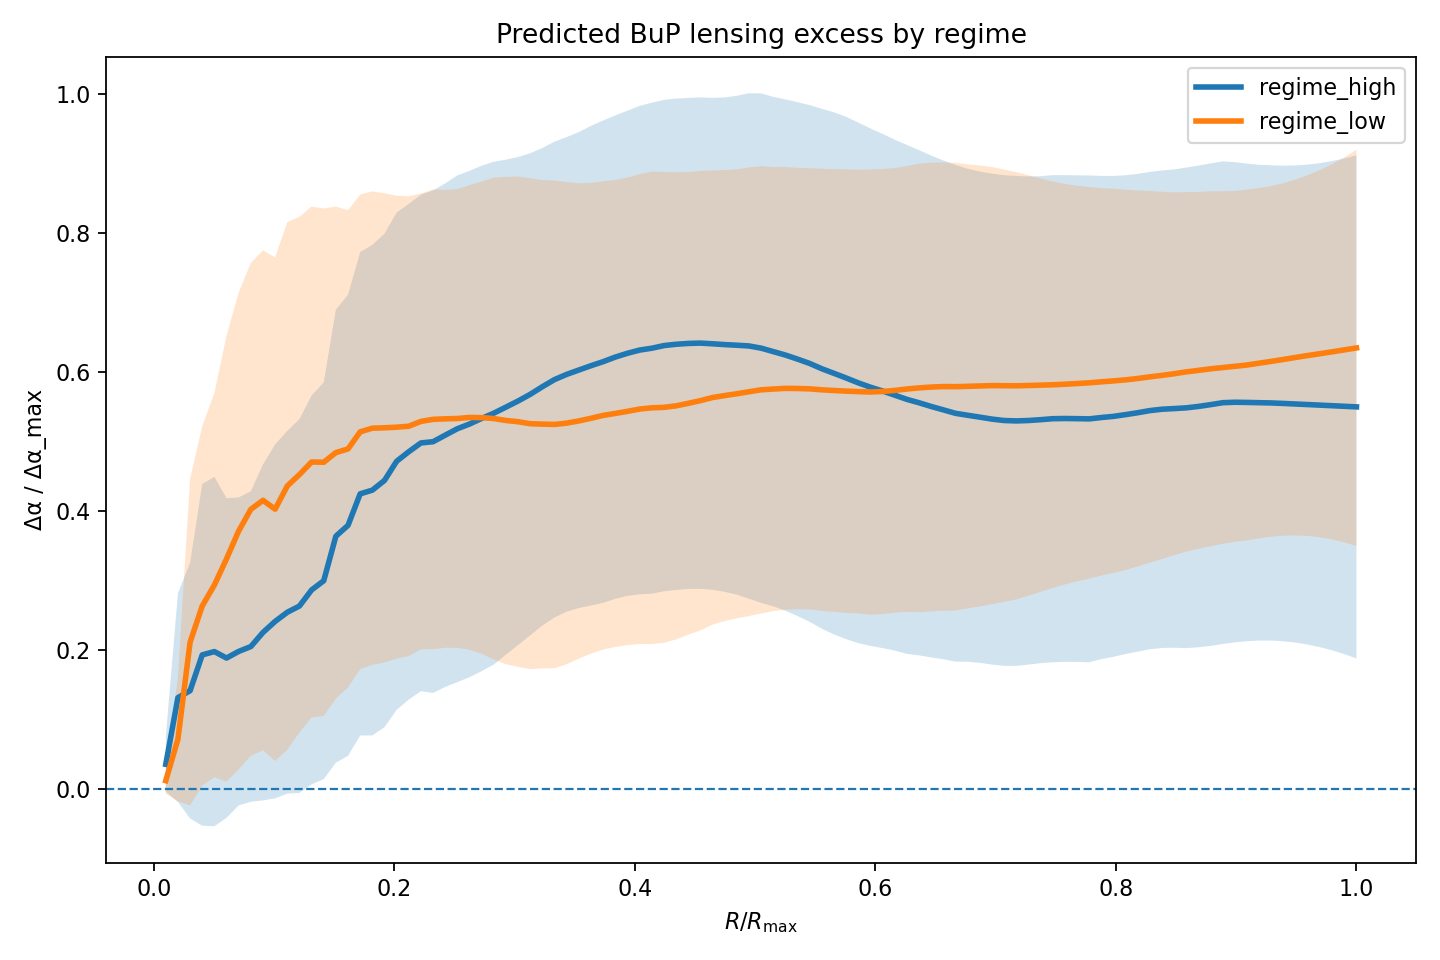
\includegraphics[width=0.7\textwidth]{lensing_regime_profiles.png}
\caption{Profil moyen de l'excès de lentillage BuP selon le régime galactique.}
\end{figure}

\subsection{Prédiction de lentillage}

À partir des profils ajustés, nous construisons un proxy de déflexion

\[
\alpha(R) \propto \frac{v(R)^2}{R}.
\]

Nous définissons

\[
\Delta \alpha(R) = \alpha_{\mathrm{BuP}}(R) - \alpha_{\mathrm{bary}}(R).
\]

Pour chaque galaxie, nous extrayons la position du maximum

\[
x_{\mathrm{peak}} = \frac{R_{\mathrm{peak}}}{R_{\max}}.
\]

Sur 102 galaxies, nous obtenons :

\begin{itemize}
\item régime LOW : $x_{\mathrm{peak}} \approx 0.365$
\item régime HIGH : $x_{\mathrm{peak}} \approx 0.498$
\end{itemize}

Donc

\[
x_{\mathrm{peak}}^{\mathrm{LOW}} < x_{\mathrm{peak}}^{\mathrm{HIGH}}.
\]

\begin{figure}[h]
\centering
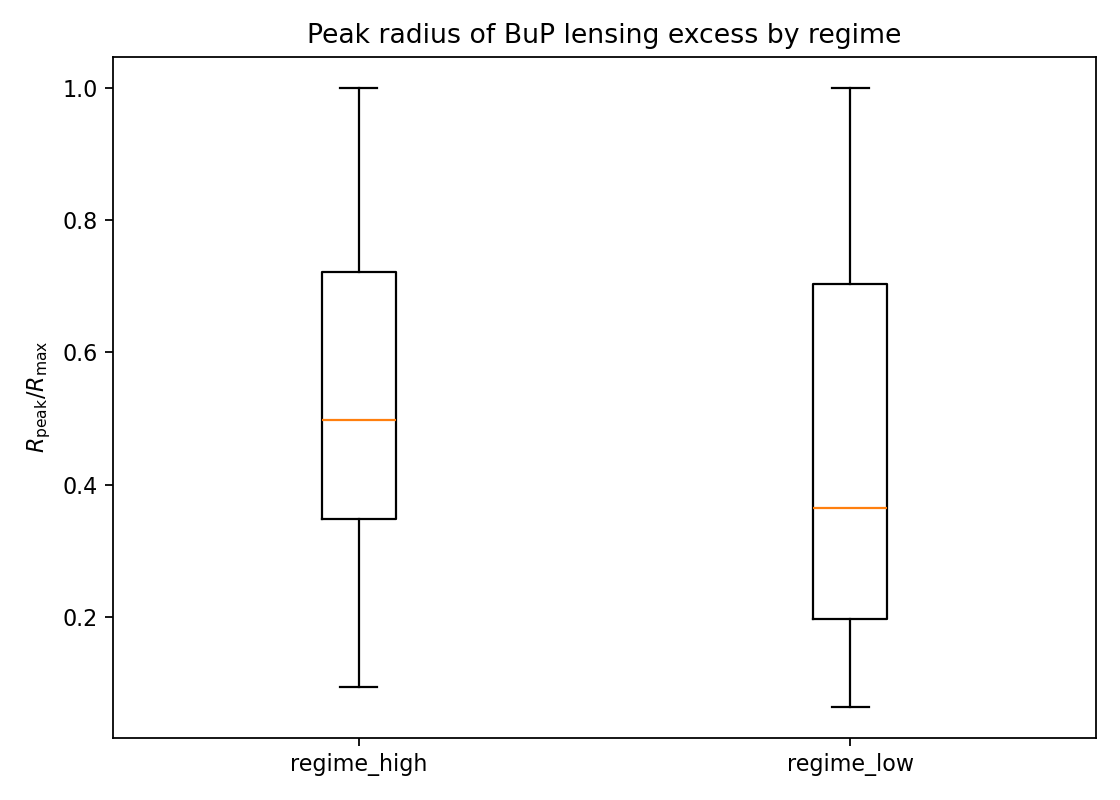
\includegraphics[width=0.6\textwidth]{lensing_peak_radius_boxplot.png}
\caption{Distribution de $R_{\mathrm{peak}}/R_{\max}$ selon le régime galactique.}
\end{figure}

\subsection{Interprétation}

Le cadre BuP prédit que :

\begin{itemize}
\item régime LOW : géométrie plus flexible, effet centralisé
\item régime HIGH : géométrie plus étalée, effet distribué
\end{itemize}

\subsection{Implication physique}

Ce résultat constitue une prédiction falsifiable indépendante des courbes de rotation. À masse baryonique comparable, la structure radiale du lentillage dépend du régime galactique.

\subsection{Comparaison avec les interprétations basées sur la matière noire}

Le cadre BuP étudié ici diffère conceptuellement des modèles standards à halo sombre. L'excès gravitationnel n'est pas attribué à une masse invisible additionnelle, mais à une modification de la géométrie émergente elle-même, encodée phénoménologiquement via une dimension effective et une échelle de transition $r_{\mathrm{trans}}$.

Les résultats sur le proxy de lentillage renforcent cette distinction. Nous trouvons que la position radiale normalisée du pic de l'excès de déflexion diffère systématiquement entre les deux régimes :

\[
\left(\frac{R_{\mathrm{peak}}}{R_{\max}}\right)_{\mathrm{LOW}}
<
\left(\frac{R_{\mathrm{peak}}}{R_{\max}}\right)_{\mathrm{HIGH}}.
\]

Le point discriminant n'est donc pas seulement la possibilité de reproduire certaines courbes de rotation, mais la prédiction de profils de lentillage qui diffèrent systématiquement des attentes issues des modèles à halo sombre.

\subsection{Synthèse}

La séparation en régimes observée dans les courbes de rotation se propage à des observables de lentillage, renforçant l'interprétation d'une description effective multi-phase de la géométrie émergente.

% =====================================================================
% PARTIE X : SYNTHÈSE ET PERSPECTIVES
% =====================================================================

\section{Ce que le Cadre Établit}

\begin{itemize}
\item la géométrie peut émerger d'états quantiques finis,
\item la dimension spatiale dépend de la structure d'intrication,
\item la dynamique modulaire est chaotique avec des signatures RMT universelles,
\item la constante modulaire $C=d_A g_2^{\mathrm{plateau}}$ encode l'information topologique,
\item les signatures ER=EPR deviennent mesurables opérationnellement,
\item des régions de type horizon émergent via des goulots d'étranglement informationnels,
\item un algorithme de détection bottom-up identifie ces régions (rang 2/55 en mode horizon-aware),
\item les corrélations multipartites présentent une structure géométrique triangulaire locale,
\item une perturbation informationnelle locale induit une réponse positive de courbure d'Ollivier--Ricci,
\item cette réponse croît avec l'intensité de la perturbation et se localise davantage pour les défauts compacts,
\item la connexion de jauge discrète $R_{ij} \in SO(3)$ est un observable géométrique sensible à la symétrie du vide,
\item une symétrie résiduelle effective U(1)-like est observée numériquement dans le vide anisotrope,
\item cette sélection d'axe est robuste vis-à-vis du paramètre kNN ($k=1..7$) et du niveau de désordre ($h \lesssim 0.2$),
\item le vide est unique : dispersion angulaire $\Delta_{\mathrm{vide}} = 0.056$ rad (normalisé : $0.072$),
\item les Hamiltoniens modulaires sont quasi-locaux ($R^2 \geq 0.99$ pour les états structurés) et amplifient l'anisotropie microscopique de façon état-dépendante,
\item une première extension phénoménologique vers les courbes de rotation SPARC suggère une description en régimes effectifs distincts,
\item la dimension émergente acquiert un rôle potentiel d'observable phénoménologique à l'échelle galactique,
\item une loi d'échelle pour $r_{\mathrm{trans}}$ est identifiée, avec une séparation en deux régimes selon la compacité baryonique,
\item cette structure d'échelle se propage aux observables de lentillage, produisant une prédiction falsifiable.
\end{itemize}

\section{Limites}

\begin{itemize}
\item limite continue $N\rightarrow\infty$ non encore établie,
\item dynamique relativiste complète absente,
\item équations d'Einstein non dérivées des premiers principes,
\item tailles de système finies limitent les claims d'universalité,
\item la symétrie U(1)-like effective résulte d'une brisure explicite et non spontanée,
\item le couplage matière--courbure est établi comme preuve de concept numérique, pas encore comme loi fondamentale dérivée,
\item l'analyse SPARC reste exploratoire et ne constitue pas encore un modèle galactique complètement contraint,
\item les diagnostics en $\chi^2$ indiquent qu'un travail supplémentaire de calibration et de sélection de modèle reste nécessaire,
\item le lentillage est traité au niveau d'un proxy radial, et non encore d'une métrique optique relativiste complète.
\end{itemize}

\section{Perspectives}

Les directions futures incluent

\begin{itemize}
\item scaling à taille finie vers $N>25$ (32, 36 qubits),
\item connexions avec les modèles chaotiques de type SYK,
\item analyse de dimension spectrale multi-échelle,
\item dérivation d'une loi effective matière--courbure sur graphe,
\item implémentations sur simulateur quantique,
\item raffinement du diagramme de phase galactique sur l'échantillon SPARC,
\item confrontation avec d'autres observables astrophysiques : relations baryoniques, lentillage, profils de masse,
\item dérivation d'un pipeline complet $d(r)\rightarrow$ métrique optique effective $\rightarrow \alpha(R)$,
\item test observationnel des prédictions de lentillage sur les échantillons SLACS et futurs relevés (Euclid, Rubin),
\item extension de l'étude des Hamiltoniens modulaires à des états construits à partir de la dynamique variationnelle BuP.
\end{itemize}

% =====================================================================
% CONCLUSION
% =====================================================================

\section{Conclusion}

La Gravité Quantique Bottom-Up propose que la géométrie spatio-temporelle peut émerger de la structure d'intrication des états quantiques sans aucun arrière-plan géométrique préalable.

Même de petits systèmes quantiques ($N=9,16$) présentent de multiples signatures cohérentes :

\begin{itemize}
\item dimension émergente ajustable par la localité de l'intrication,
\item dynamique modulaire chaotique avec constante $C$ dépendante de la topologie,
\item raccourcis opérationnels ER=EPR,
\item goulots d'étranglement informationnels de type horizon détectables algorithmiquement,
\item gravité thermodynamique approximative via une relation entropie-énergie de type Jacobson,
\item réponse locale de la courbure d'Ollivier--Ricci à une perturbation informationnelle,
\item première extension phénoménologique aux galaxies SPARC,
\item identification d'une structure d'échelle pour $r_{\mathrm{trans}}$ et séparation en deux régimes,
\item prédiction falsifiable sur les observables de lentillage.
\end{itemize}

\bigskip

Un résultat complémentaire important concerne la structure interne du vide effectif du modèle Bottom-Up. Nos analyses montrent que ce vide ne se comporte pas comme un milieu isotrope trivial, mais comme un milieu structuré dont les propriétés dépendent de l'anisotropie des interactions et du niveau de désordre local. En particulier, nous observons la sélection robuste d'une symétrie effective de type U(1), associée à la sélection d'une direction privilégiée dans l'espace des générateurs locaux de la connexion de jauge émergente.

Cette symétrie résiduelle n'est pas le résultat d'une brisure spontanée au sens des théories de champs --- les champs locaux et l'anisotropie $J_{zz} \neq J_{xy}$ brisent explicitement $SO(3)$ au niveau du Hamiltonien. Elle résulte d'une \textbf{sélection robuste d'un axe effectif} par l'état fondamental, dont la robustesse vis-à-vis des choix de reconstruction du graphe (paramètre $k \in \{1,\ldots,7\}$ des graphes kNN) indique qu'il s'agit d'une propriété intrinsèque de l'état, et non d'un artefact numérique. La transition contrôlée vers SO(3) est observée autour de $J_{zz}/J_{xy} \approx 1$ et $h \approx 0.3$.

Cette émergence est contrôlée par deux paramètres : le rapport d'anisotropie $J_{zz}/J_{xy}$ et l'amplitude du désordre local $h$. Une transition nette est observée autour de $J_{zz}/J_{xy} \approx 1$ et $h \approx 0.3$, au-delà desquels la symétrie effective redevient SO(3).

Par ailleurs, l'étude systématique des Hamiltoniens modulaires établit que $K_A$ est quasi-local ($R^2 \geq 0.99$ pour les états structurés) et amplifie l'anisotropie microscopique de façon état-dépendante ($\mathcal{A}_{\mathrm{fondamental}} = 1.048 \pm 0.114$), confirmant leur rôle de sondes géométriques de la structure d'intrication.

Ainsi, le programme Bottom-Up ne conduit pas seulement à une géométrie et une gravité émergentes, mais également à des structures de symétrie effectives et à des Hamiltoniens effectifs dérivés --- ouvrant la voie à une compréhension unifiée où géométrie, dynamique et symétrie émergent conjointement de l'organisation informationnelle des états quantiques.

\begin{thebibliography}{99}

\bibitem{jacobson}
T. Jacobson,
Thermodynamics of Spacetime,
Phys. Rev. Lett. 75, 1260 (1995).

\bibitem{vanraamsdonk}
M. Van Raamsdonk,
Building up spacetime with quantum entanglement,
Gen. Relativ. Gravit. 42, 2323 (2010).

\bibitem{maldacena}
J. Maldacena, L. Susskind,
Cool horizons for entangled black holes,
Fortschritte der Physik 61, 781 (2013).

\bibitem{pagewootters}
D. Page, W. Wootters,
Evolution without evolution,
Phys. Rev. D 27, 2885 (1983).

\bibitem{ollivier}
Y. Ollivier,
Ricci curvature of Markov chains on metric spaces,
J. Funct. Anal. 256, 810--864 (2009).

\bibitem{sparc}
F. Lelli, S. S. McGaugh, J. M. Schombert,
SPARC: Mass Models for 175 Disk Galaxies with Spitzer Photometry and Accurate Rotation Curves,
Astron. J. 152, 157 (2016).

\bibitem{Bisognano1975}
J.~J.~Bisognano and E.~H.~Wichmann,
On the duality condition for a Hermitian scalar field,
J.~Math.~Phys.\ \textbf{16}, 985 (1975).

\bibitem{Peschel2003}
I.~Peschel,
Calculation of reduced density matrices from correlation functions,
J.~Phys.~A \textbf{36}, L205 (2003).

\end{thebibliography}

\end{document}
